\documentclass[conference]{IEEEtran}

\usepackage{graphicx}
\usepackage{amsmath,amssymb}
\usepackage{textcomp,xcolor}
\usepackage{tabularx,booktabs,multirow}
\usepackage{algorithm}
\usepackage{algpseudocode}
\usepackage{cite,url,xspace}
\usepackage[hidelinks]{hyperref}
\usepackage{cleveref}
\newcommand{\sys}{\mbox{PathVeil}\xspace}
\newcommand{\pats}{\mbox{PATS}\xspace}

\begin{document}
\title{PathVeil: Learning AS Routes from Public Evidence\\without Source Measurements}
\author{\IEEEauthorblockN{Anonymous Authors}}
\maketitle

\begin{abstract}
Learning how an autonomous system (AS) reaches remote networks usually
requires observations of routes originating from that AS. Such observations
are unevenly available, leaving a source cold start for path inference.
We present \sys, a framework that constructs source-specific training
paths from other networks' routing observations and public interconnection
evidence. Its prefix-anchored tail stitching method selects likely
forwarding neighbors, resolves routing choices beyond the first hop when
necessary, and joins selected prefixes to observed route segments.
A learned complete-path scorer admits a source-specific library using
relative quality, while the same selected prefix tree constrains training
and query candidate generation. A GMPI model learns from this library to
rank candidate routes. On three monthly BGP snapshots, each containing ten target sources
and more than 685,000 query pairs, \sys obtains 82.56\%, 85.06\%, and
83.45\% AS-set Jaccard. Source-level diagnostics distinguish first-hop
coverage from complete-path observation support and expose cases where
correct first-hop sets still provide weak training paths. These results
assess route agreement under the stated limits of public evidence.
\end{abstract}

\begin{IEEEkeywords}
AS path inference, source cold start, path augmentation, interdomain routing,
public routing evidence
\end{IEEEkeywords}

\section{Introduction}
\label{sec:introduction}

Internet services depend on routes through autonomous systems (ASes) that
users and service operators do not directly control. Knowing which
networks a route traverses can help identify transit dependencies, inspect
exposure to intermediary networks, and compare connectivity to candidate
service locations~\cite{li2024internet}. These tasks require path visibility
from the network of interest, rather than only from a nearby measurement
probe. For example, a source AS $s$ may reach many destinations through one
neighbor, while the important routing choices occur at that neighbor.
Figure~\ref{fig:motivation} illustrates the problem: public observations
contain useful routes beyond $s$, but do not directly disclose which
continuations $s$ would use.

\begin{figure}[t]
\centering
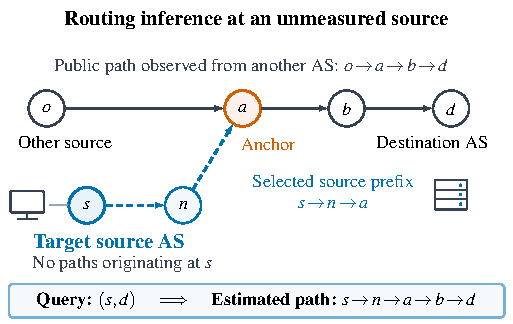
\includegraphics[width=\columnwidth]{figures/fig1_scenario.pdf}
\caption{A selected source prefix can connect an unmeasured source to a
publicly observed tail. Dashed arrows denote the inferred prefix; solid
arrows denote observed segments. Construction supplies a candidate, not
proof that the source forwards along it.}
\label{fig:motivation}
\end{figure}

Direct path measurements provide observations from deployed vantage
points. Traceroute requires a probe in, or suitable access to, the source
network; distributed platforms improve coverage but cannot guarantee that
such a probe exists for every AS~\cite{tracerouteJacobson,RIPEAtlas}.
Public BGP collectors supply routes from participating networks, whose
observations are also uneven~\cite{RouteViews,RIPERIS}.
Path inference extends this coverage, but the information it needs depends
on the method. Graph-based approaches can search for routes using public
topology and policy approximations, although these rules cannot capture
all local preferences~\cite{qiu2005path,11044440}. Stitching-based approaches
reuse observed segments but require evidence that connects the source to
those segments~\cite{probinfer}. Learning-based approaches such as
GMPI benefit from many source-rooted paths to learn source-specific
routing behavior~\cite{li2023realizing,li2024realizing}.

When observations originating from the target AS are unavailable, these
approaches face a source cold start. We address it by constructing
source-rooted training paths from routing evidence collected elsewhere.
Observed tails preserve routing decisions already made by other networks;
public interconnection information helps infer the short prefix connecting
the source to those tails. The resulting library can support learning and
candidate generation across destination queries. The aim is to infer
routes without collecting new measurements from the target source, while
making explicit which parts of a route remain inferred.

Three challenges govern this construction.
\textbf{First, where should source-specific exploration occur?}
A well-observed neighbor supplies reusable tails directly; a poorly
observed neighbor may require exploration beyond that neighbor. A source
with few neighbors can also hide substantial routing diversity at its
second hop. Selecting likely forwarding neighbors and deciding whether
to expand them therefore form one problem.
\textbf{Second, how should paths be constructed and admitted?}
A graph route can satisfy coarse policy rules without reflecting an
observed routing decision. Stitching retains observed decisions, but an
otherwise plausible join can still produce a route that the source would
not use. Candidate construction must be coupled with complete-path
assessment, and the admitted library must be examined for concentration
on a few easy branches.
\textbf{Third, how can heterogeneous public evidence support these
choices?} Relationships, topology, BGP segments, and co-location metadata
have different meanings and coverage. They must inform AS, prefix, and
path representations without treating missing information as a negative
observation or shared facilities as established links.

We present \textbf{\sys}, whose core method is
\textbf{prefix-anchored tail stitching (\pats)}.
\textbf{For the first challenge,} source-topology-conditioned prefix
selection combines learned neighbor ranking with bounded exploration.
A source-shape statistic compares distinct two-hop reachability with
first-hop degree. For one regime, usable-tail capacity determines whether
to explore further; for the other, every selected first hop is expanded
to resolve downstream choices. The output retains complete prefixes and
their commercial-phase context, forming one source-specific tree shared
by subsequent stages.

\textbf{For the second challenge,} observed-tail construction and learned
quality admission connect short selected prefixes to intact forward
segments. This reuses much of an existing routing decision instead of
inventing the full route. A complete-path model assesses support using
prefix, segment, and destination context. Admission uses a source-relative
score threshold with an explicit minimum-library rule. During inference,
the selected tree anchors both observed tails and topology-derived
alternatives. This design controls where routes can leave the source;
it does not assume that a quality threshold alone guarantees branch
representation.

\textbf{For the third challenge,} a multilevel evidence representation
encodes network attributes and co-location, directed transitions and
commercial phases, and complete-path support. Destination-conditioned
features compare observations across independent donor sources, with
per-donor normalization to reduce domination by prolific observers.
Unknown relationships and missing evidence remain explicit. The admitted
path set supplies both source-specific training labels and local path
knowledge for candidate generation, keeping these consumers consistent.
We use GMPI as the downstream ranking model without changing its
architecture or learning objective.

Our contributions are:
\begin{itemize}
\item A framework for source-cold-start AS route inference that builds
source-specific learning evidence from public observations and
interconnection metadata, without requiring measurements originating
from the target source as an input.
\item A prefix-anchored path-augmentation method that combines
source-topology-conditioned exploration, reuse of observed tails, and
complete-path quality admission, with one prefix tree shared by training
and query generation.
\item An evaluation of constructed-source inference on fixed BGP query
cohorts, with source-level results and distinct criteria for prefix
selection, augmented-path observation support, and final route agreement.
The evaluation distinguishes representation through selected neighbors
from complete-path observation support and final AS-set agreement.
\end{itemize}

\section{Background and Related Work}
\label{sec:background}

\subsection{Routing Observations and Their Limits}

BGP separates learning a route from a neighbor, selecting a route under
local policy, and exporting it to other neighbors~\cite{rfc4271}.
Consequently, an observation of $(n,\ldots,d)$ does not establish that
$n$ exports that route to source $s$, or that $s$ selects it.
Route Views and RIPE RIS expose advertised AS paths from participating
networks~\cite{RouteViews,RIPERIS}. CAIDA relationships and ASRank add
commercial roles, connectivity, and customer-cone attributes;
PeeringDB supplies self-reported network and interconnection
metadata~\cite{caidaASRelationships,caidaASrank,PeeringDB}.
These sources constrain plausible routing but do not reveal private
preferences. Shared IXP or facility presence does not prove adjacency.
Valley-free compatibility describes a common commercial model, not a
complete account of operational policy~\cite{gao2001inferring}.

Traceroute discovers responding hops by varying IP time-to-live.
Classic traceroute can combine replies from multiple paths under load
balancing; Paris traceroute controls flow identifiers to reduce per-flow
artifacts~\cite{tracerouteJacobson,ParisTraceroute}.
Scamper supports parallel, rate-controlled measurement, and RIPE Atlas
provides distributed probes~\cite{scamper2010,RIPEAtlas}.
Their output still depends on source placement, filtering, and responding
routers. Unresponsive hops leave gaps, and IP-to-AS conversion introduces
additional ambiguity~\cite{RIPEAtlasResultFormat,mao2003AStraceroute}.
A traceroute data-plane observation and a BGP control-plane path are
related evidence, rather than interchangeable ground truth.

\subsection{AS Path Inference}

\textbf{KnownPath} uses BGP paths as anchors for inferring source-to-prefix
routes under routing constraints~\cite{qiu2005path}.
\textbf{ProbInfer} represents observed path segments in a multigraph,
composes candidates, and evaluates them probabilistically~\cite{probinfer}.
These approaches demonstrate the value of preserving observed segments;
their source connectivity still depends on the available anchors and
policy assumptions.

\textbf{GMPI} combines heuristic path generation with a neural evaluation
model that integrates AS attributes, topology, and related observed paths
through path representations and attention~\cite{li2023realizing}.
\textbf{PA-GMPI} adds personalized generation and adaptive training,
including a graph-kernel warm starter and representations learned from
observed walks~\cite{li2024realizing}.
Both motivate source-specific learning, while their training observations
are an important resource requirement. \sys supplies constructed
source-specific evidence and a common prefix constraint; GMPI provides
the downstream candidate score.

\textbf{PathRadar} distinguishes core and shell ASes using routing
complexity and observation adequacy, combining policy-based and
stitching-based inference. Progressive learning propagates candidate
routes and addresses prefix-specific and multiple-path
inference~\cite{11044440}.
Its treatment of heterogeneous observation conditions is related to our
exploration decision. Our method uses a selected source prefix tree and
complete-path admission to build a reusable training library.

Other systems address adjacent objectives. iPlane composes measured
segments to predict paths and their properties~\cite{madhyastha2006iplane,madhyastha2009iplane};
PredictRoute combines historical control- and data-plane evidence for
probabilistic prediction~\cite{singh2021predictroute}; RouteInfer models
commonality and diversity in ISP routing~\cite{wang2022routeinfer}.
A broader survey reviews the applications and limitations of interdomain
path inference~\cite{li2024internet}.
These works provide context for our focus: learning routes for a target
source whose own originating observations are unavailable to construction.

\section{Problem Setting and Evidence Roles}
\label{sec:problem}

\subsection{Source-Cold-Start Queries}

A query specifies a source AS $s$, destination AS $d$, and snapshot $t$.
We return an ordered forward AS sequence $\widehat P_{s,d}$, or no usable
estimate. The source need not host a probe or contribute source-originated
paths to the construction input. Observations from other origins may
contain $s$ internally; they remain indirect public evidence. We never
reverse an observation to manufacture a forward route.

The AS-pair abstraction pools destination prefixes within an AS.
Different prefixes can follow different routes, so one returned sequence
is an estimate rather than a guarantee for every packet or endpoint.
For a service query, resolving an endpoint and mapping its prefix to $d$
precedes our inference; DNS steering and anycast can change that
endpoint or its serving instance~\cite{schomp2020akamai,koch2021anycast}.
We do not infer the return path, router sequence, geography, or latency.

\subsection{Public Evidence and Supervision}

We distinguish four roles. Public background paths supply topology and
reusable observed segments. Reference paths from separate training
origins supervise the neighbor and path-support models. Augmented paths
form the target source's downstream training library. Finally, held-out
source routes label final evaluation queries and do not supervise target
construction or checkpoint selection.

Let $\mathcal G_t$ be the public AS graph and $\mathcal P_{\rm pub}$ the
permitted background path corpus. A path $P=(v_0,\ldots,v_\ell)$ supplies
a forward tail $(v_i,\ldots,v_j)$ for $i<j\leq\ell$.
A selected prefix $q=(s,\ldots,v_i)$ joins that tail at $v_i$, including
the anchor once. Reuse preserves the observed order. An internal endpoint
$j<\ell$ is allowed; it supplies evidence to the AS at that endpoint.
Training-donor observations additionally support destination-context
features and inference candidates under their own origin restrictions.
These roles are not merged simply because two files contain the same AS.
Table~\ref{tab:data_sources} summarizes the external data.

\begin{table*}[t]
\centering
\caption{External data and their roles. Monthly snapshots refer to
February 1, March 1, and April 1, 2026. Evidence and final reference labels
have separate consumers.}
\label{tab:data_sources}
\small
\setlength{\tabcolsep}{4pt}
\begin{tabularx}{\textwidth}{@{}p{3.0cm}p{2.7cm}X@{}}
\toprule
Source & Snapshot / period & Contents and use\\
\midrule
Route Views / RIPE RIS~\cite{RouteViews,RIPERIS}
& Three monthly dates; Oct.\ 15
& Public AS paths for topology, observed segments, and separately
partitioned upstream supervision. Designated source routes label the
fixed BGP query cohorts. Inherited graph-feature provenance is discussed
in the evaluation protocol.\\
CAIDA relationships~\cite{caidaASRelationships}
& Three monthly dates; Oct.\ 1
& Directed provider--customer and peer roles for AS/prefix/path features
and commercial-phase checks. Missing roles remain unknown.\\
CAIDA ASRank~\cite{caidaASrank}
& Three monthly dates; Oct.\ 1
& AS and link attributes, including rank, degree, and customer-cone size,
for neighbor ranking and public graph representation.\\
PeeringDB~\cite{PeeringDB}
& Three monthly dates; Oct.\ 14
& Network attributes and IXP/facility memberships for candidate retrieval
and co-location features; shared presence does not establish adjacency.\\
\midrule
Tranco N26XW~\cite{lepochat2019tranco}
& Oct.\ 14
& Frozen one-million-domain list for the independent endpoint dataset.\\
DNS resolution (this study)
& Oct.\ 15
& 911,257 resolved domains; 388,491 unique IPv4 probe targets.\\
CAIDA prefix-to-AS~\cite{caidaRouteviewsPfx2AS}
& Oct.\ 13, 10:00 UTC
& Longest-prefix origin mapping for endpoints and responding hops;
ambiguous mappings do not become certain labels.\\
Traceroute (this study)
& Oct.\ 15--16
& AS63835: 388,491 TCP and 243,207 ICMP Paris records. Filtering yields
2,198 distinct ordered AS paths over 1,890 pairs for evaluation only.\\
\bottomrule
\end{tabularx}
\end{table*}


\subsection{Library and Inference Objective}

Construction produces a selected prefix tree $\mathcal T_s$ and an
admitted library $\mathcal L_s$. The tree retains the source, each chosen
first hop, any explored second hop, and feasible commercial-phase states.
Both training and query candidate generation use this complete tree.
The same ordered path set $\mathcal L_s$ provides downstream training
labels and local path knowledge, verified by a common path-set hash.

For candidate set $\mathcal C_{s,d}$ and available history $H_{s,d}$,
query inference selects
\begin{equation}
\widehat P_{s,d}=\underset{P\in\mathcal C_{s,d}}{\arg\max}
 f_{\theta_s}(P,H_{s,d}).
\label{eq:query_score}
\end{equation}
The source model $f_{\theta_s}$ is trained on $\mathcal L_s$.
The complete-path admission score and the query score in
\eqref{eq:query_score} serve different decisions; neither is interpreted
as a calibrated probability of actual forwarding.

\section{Methodology}
\label{sec:method}

\subsection{Framework Overview}

\begin{figure*}[t]
\centering
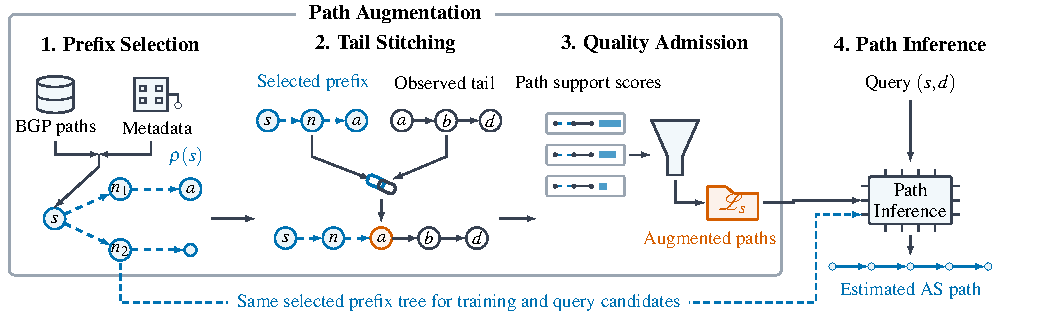
\includegraphics[width=\textwidth]{figures/fig2_overview.pdf}
\caption{\sys constructs a source-specific prefix tree, joins its prefixes
to observed tails, and selects an augmented path library. The same complete
tree constrains candidate generation during model training and inference;
the admitted library supplies both training labels and local path knowledge.}
\label{fig:overview}
\end{figure*}

\sys addresses source cold start by transferring routing evidence from
other networks. Its augmentation procedure, \pats (Prefix-Anchored Tail
Stitching), first selects likely forwarding neighbors and determines
whether to explore their next hops. It then joins the resulting prefixes
to intact observed tails and assesses the complete constructed routes.
The resulting library trains a source-specific inference model without
opening the source's held-out route labels. Figure~\ref{fig:overview}
shows the separation between path augmentation and final inference.

Two objects are retained for each source: the complete selected prefix
tree $\mathcal T_s$ and the admitted path library $\mathcal L_s$. They serve different
purposes. The tree defines the permitted early forwarding choices; the
library provides surrogate training routes and local path knowledge.
Candidate generation uses the complete tree, including selected prefixes
that do not happen to dominate the admitted library. Thus library
selection cannot silently redefine the source's permitted exits.

\subsection{Representing Heterogeneous Routing Evidence}
\label{sec:representation}

We represent public AS relationships and ASRank attributes,
PeeringDB presence, and independent BGP observations at AS-pair,
transition, and complete-path levels~\cite{CAIDA,caidaASrank,PeeringDB}.
Table~\ref{tab:method_features} summarizes their roles. Features are
tabular, with explicit missingness and conflict indicators. Shared
PeeringDB IXPs or facilities identify potential interconnection partners;
co-location alone does not establish a physical link or an export policy.

\begin{table}[t]
\centering
\caption{Evidence representations and their computational roles. Missing
and conflicting observations remain explicit.}
\label{tab:method_features}
\footnotesize
\begin{tabularx}{\columnwidth}{@{}lX@{}}
\toprule
Representation & Features and use\\
\midrule
AS pair & Public adjacency and commercial roles; ASRank degree, cone,
and network attributes; PeeringDB IXP/facility overlap and population;
independent edge support. Neighbor retrieval and ranking.\\
Graph structure & Common-neighbor overlap, Adamic--Adar,
resource allocation, role-conditioned bridges; source first- and
second-layer size. Structural ranking and $\rho(s)$.\\
Prefix/transition & Preceding, current, and next AS; local rank and
presence scores; edge provenance and possible commercial phases.
Conditional exploration and prefix-state tracking.\\
Path evidence (181) & Ordered path, suffix, edge and destination
support; AS count and commercial-role sequence; public endpoint context.
Base features for complete-path scoring.\\
Prefix reliability (32) & Support/missingness across added edges,
inferred-edge fraction, feasible phase states, and soft first-hop
transit-role evidence.\\
Actual next hop (9) & Conditional support, rank, missingness, and
phase status of the candidate's actual third AS.\\
Destination context (33) & Donor-source agreement and equally weighted
route fractions at the first hop and stitching boundary, with incoming-role
conditioning and explicit absent-boundary indicator.\\
\bottomrule
\end{tabularx}
\end{table}


\paragraph{Separating evidence from supervision.}
The upstream procedure masks complete observations by their original
first ASN before expanding paths into segments. Independent background
observations provide ordered edges and forward contiguous segments.
Task-source observations have separate roles: training origins provide
supervised labels and destination-conditioned donor statistics, while
held-out origins provide evaluation labels. A segment containing $s$
inside another origin's observation can remain evidence; an observation
originally rooted at held-out $s$ is excluded from this upstream evidence.
Tails preserve their observed direction and are never constructed by
reversing a route. These upstream guarantees apply to the explicitly
masked corpus; the provenance of inherited downstream graph and embedding
artifacts is assessed separately in the experimental protocol.

\paragraph{Destination-conditioned transfer.}
A path observed at an intermediate AS need not be exported to a particular
neighbor~\cite{rfc4271}. We therefore complement segment support with
evidence about which next hops other receivers observe toward the same
destination. For an original training donor $v$, let $c_v(n,a,d)$ count
distinct complete routes beginning $(v,n,a)$ and ending at $d$, and let
$c_v(n,d)=\sum_b c_v(n,b,d)$. With
$V_{n,d}=\{v:c_v(n,d)>0\}$, two representative features are
\begin{equation}
\begin{split}
f(n,a,d)&=\frac{|\{v\in V_{n,d}:c_v(n,a,d)>0\}|}{|V_{n,d}|},\\
m(n,a,d)&=\frac{1}{|V_{n,d}|}\sum_{v\in V_{n,d}}
                         \frac{c_v(n,a,d)}{c_v(n,d)}.
\end{split}
\label{eq:destination_evidence}
\end{equation}
The first measures agreement across donors and the second gives every
donor equal weight after normalizing its alternative routes. We also
condition these statistics on the donor's incoming commercial role at
$n$, matching the candidate receiver's role when it is known. This uses
original receiver contexts, rather than treating every internal occurrence
of $n$ as an independent receiver observation.

These features are evaluated at both the first-hop transition and the
construction boundary. Two 16-column context vectors and one boundary
indicator add 33 columns to 181 path-evidence, 32 prefix-reliability,
and nine actual-next-hop columns, giving a 255-column complete-path
representation. Missing donor coverage remains explicit. For a training
source, the entire original-source fold is removed from its donor
statistics, even when recursion changes the stitching anchor.

\subsection{Source-Conditioned Neighbor Selection and Exploration}
\label{sec:prefix_selection}

\paragraph{Learning likely forwarding choices.}
Candidate neighbors are retrieved from public or independently observed
adjacency and PeeringDB co-location, with graph-supported candidates
prioritized in a pool of at most 4,096 ASes. Two LightGBM
rankers~\cite{ke2017lightgbm} use a public-evidence view and a structurally
extended view. The latter adds common-neighbor overlap, Adamic--Adar,
resource-allocation, and population-weighted IXP/facility features.
Each view also has a binary presence head.

Training first-hop importance gives each destination equal weight,
divided among its distinct observed routes. Observed neighbors ranked
1--3, 4--10, and beyond ten receive relevance labels
3, 2, and 1; unobserved candidates receive 0. Presence indicates use in
this finite reference corpus. These targets measure observed routing
choices, rather than link existence or traffic volume.

Let $r_s^{\mathrm{pub}}(n),r_s^{\mathrm{str}}(n)$ denote the ranker outputs
and $p_s^{\mathrm{pub}}(n),p_s^{\mathrm{str}}(n)$ the presence outputs.
The protected core is
\begin{equation}
K_s=\operatorname{Top}_3(r_s^{\mathrm{pub}})
       \cup\operatorname{Top}_3(r_s^{\mathrm{str}}).
\label{eq:protected_core}
\end{equation}
For ordering within the core and the remaining candidates, we use
\begin{equation}
\begin{split}
\bar p_s(n)&=\tfrac12\bigl(p_s^{\mathrm{pub}}(n)+p_s^{\mathrm{str}}(n)\bigr),\\
u_s(n)&=z(r_s^{\mathrm{str}}(n))+
                   0.5\log\frac{\bar p_s(n)}{1-\bar p_s(n)},
\end{split}
\label{eq:neighbor_ranking}
\end{equation}
where $z$ standardizes within the candidate pool and presence outputs
are clipped to $[10^{-6},1-10^{-6}]$ before taking the logit.
The core precedes the remaining candidates, with descending $u_s$ and
ASN tie breaking. Presence outputs are uncalibrated observation-support
scores; we do not interpret them as forwarding probabilities.

\paragraph{Adapting exploration to source structure.}
Degree alone misses a source whose first hop conceals a large next-layer
choice set. Let $b_1(s)$ be the source's public degree, and let $b_2(s)$
count distinct second-layer ASes reachable through loop-free,
commercially non-incompatible two-hop public prefixes. Unknown roles
remain eligible. We define
\begin{equation}
\rho(s)=\frac{b_2(s)}{b_1(s)^2}.
\label{eq:source_rho}
\end{equation}
This is a structural control statistic, not a routing probability.
It is computed once for the original source and is not recomputed to
switch policies at its neighbors. A source with no usable public degree
remains unresolved.

When $\rho(s)\leq1$, we select the longest prefix of the protected-core
ordering containing $K_s$, limited to a root budget $\kappa$, whose mean
$\bar p_s$ is at least 0.7. If none qualifies, the core is retained with
uncertain support. For each selected neighbor $n$, we count usable
independent forward tails for $(s,n)$, stopping once 300 are found.
A usable direct prefix is retained. If its capacity is below 300,
exploration also proposes $(s,n,a)$ prefixes.
An explored child is retained only if it has at least one usable tail.
The evaluated protocol uses $\kappa=21$, the 90th-percentile number of
first-hop neighbors needed to cover 80\% of original training paths in
the February source statistics. This is a search budget, not a
guarantee of reference coverage for a new source.

When $\rho(s)>1$, only the dual-ranker core $K_s$ is selected, yielding
at most six roots. Every root is expanded to $(s,n,a)$ independently
of its direct-tail capacity. This exposes choices hidden behind a narrow
first layer; the high-$\rho$ branch does not retain a broad direct-tail
bypass. Both policies use the same next-hop width of ten and a maximum
prefix length of three ASes.

\paragraph{Prefix-aware next-hop prediction.}
A conditional ranker uses the preceding AS, current AS, and candidate
next AS to transfer local routing preferences. Its candidate pool is
limited to 512. Each proposed extension must avoid visited ASes and have
independent/public edge evidence, or co-location accompanied by a finite
learned support score. It must also preserve at least one feasible
commercial phase of the complete prefix. We track upward, post-peer,
and downward states; sibling edges are neutral and unknown relationships
retain all feasible states. Distinct prefixes and phase states sharing
an anchor remain distinct. This is local conditional transfer, not a
claim that multiplying local scores gives a calibrated path probability.
No supported continuation means stopping that branch rather than
inventing an extension.

\subsection{Prefix-Anchored Tail Construction}
\label{sec:construction}

For each selected prefix $q=(s,\ldots,z)$, \pats joins it to an intact
observed forward tail $t=(z,\ldots,d)$:
\begin{equation}
q\oplus t=(s,\ldots,z,\ldots,d),
\label{eq:pats_join}
\end{equation}
including the common anchor $z$ once. Reusing a tail preserves multiple
consecutive observed routing choices. It does not establish that $s$
would learn or select the resulting route.

Construction checks valid ASNs, 3--20 ASes, absence of loops, support
for each added prefix edge, and existence of a valley-free assignment
consistent with known relationships~\cite{gao2001inferring}. Missing
relationships are retained as unknown rather than automatically rejected.
The same physical path may arise from different prefixes; ordered
sequences are deduplicated while retaining their construction provenance.

To bound scoring work while preserving alternatives, construction keeps
up to two evidence-prioritized candidates per first hop, actual third AS,
destination, and AS count. It favors fewer unobserved prefix extensions
and stronger independent segment support. A deterministic hash ordering
selects 5,000 destination contexts, supplemented by all destinations of
direct prefixes covering at most 1,000 destinations and up to 50 protected
destinations per other explicit prefix. These are construction work
budgets, not a final library-size cap.

\subsection{Complete-Path Scoring and Library Admission}
\label{sec:admission}

\paragraph{Learning finite-observation support.}
A LightGBM classifier $h_\theta(\phi(P))$ assesses the 255-column
representation of a complete constructed path. For a training source,
an exact ordered match to its original reference is positive. A
nonmatching candidate is negative only if its destination has reference
coverage; candidates for uncovered destinations remain unlabeled.
The weighted binary objective balances training sources, first hops,
destinations within first hops, and alternatives within each context.
The model uses 300 trees, at most 31 leaves per tree, maximum depth seven,
and learning rate 0.04.

Models are fitted separately for each date using registered training
origins. Neighbor and transition predictions for a training source use
heads fitted without its original-source fold; destination features
exclude the same fold. This is stagewise source isolation. The final
path classifier is fitted on these training cases, and held-out source
routes never determine its features or parameters. Because non-observation
does not prove route impossibility, $h_\theta$ estimates support in a
finite observation corpus, rather than the probability of forwarding
reality.

\paragraph{Source-relative admission.}
Let $\mathcal B_s$ be the legal deduplicated source candidate pool and
$q(P)=h_\theta(\phi(P))$. We normalize within that source:
\begin{equation}
\widetilde q_s(P)=\frac{q(P)}{\max_{P'\in\mathcal B_s}q(P')}.
\label{eq:relative_quality}
\end{equation}
The nominal threshold is 0.75. To retain at least 1,000 paths when
positive-scored capacity permits, let $\widetilde q_{s,(1000)}$ be the
1,000th highest relative score and set
\begin{equation}
\begin{split}
\tau_s&=\min\{0.75,\widetilde q_{s,(1000)}\},\\
\mathcal L_s&=\{P\in\mathcal B_s:\widetilde q_s(P)\geq\tau_s\}.
\end{split}
\label{eq:quality_admission}
\end{equation}
All cutoff ties are retained and there is no upper size cap. The library
is unresolved if fewer than 1,000 legal paths exist, if the required
cutoff is zero, or if the source maximum is zero. The threshold relaxation
and actual cutoff are recorded. Relative quality is an admission ranking
criterion, not a guarantee of 75\% route accuracy. Algorithm~\ref{alg:path_synthesis}
summarizes augmentation.

\begin{algorithm}[t]
\caption{Prefix-Anchored Tail Stitching and Admission}
\label{alg:path_synthesis}
\footnotesize
\begin{algorithmic}[1]
\Require Source $s$, public topology $G$, independent tails $\mathcal T$
\Require Neighbor heads $g$, conditional ranker $g_c$, path scorer $h_\theta$
\Require Root budget $\kappa$ ($21$ in the evaluated protocol)
\Ensure Prefix tree $\mathcal T_s$ and admitted library $\mathcal L_s$, or unresolved
\If{$b_1(s)=0$}
  \State \Return unresolved
\EndIf
\State $\rho\gets b_2(s)/b_1(s)^2$
\State $K\gets\operatorname{Top}_3(g_{\rm pub}(s))\cup\operatorname{Top}_3(g_{\rm str}(s))$
\If{$\rho\leq1$}
  \State $N\gets\Call{ProtectedSupportPrefix}{s,K,\kappa,0.7}$
\Else
  \State $N\gets K$
\EndIf
\State $Q\gets\emptyset$
\ForAll{$n\in N$}
  \State $q\gets(s,n)$; $c\gets\Call{UsableTailCount}{q,\mathcal T,300}$
  \If{$\rho\leq1$ and $c>0$}
    \State $Q\gets Q\cup\{q\}$
  \EndIf
  \If{$\rho>1$ or $c<300$}
    \State $A\gets\Call{SupportedTopK}{g_c(s,q),10}$
    \ForAll{$a\in A$ with $a\notin q$}
      \State $q'\gets q\mathbin{\|}(a)$
      \If{$\rho>1$ or $\Call{UsableTailCount}{q',\mathcal T,1}>0$}
        \State $Q\gets Q\cup\{q'\}$
      \EndIf
    \EndFor
  \EndIf
\EndFor
\State $\mathcal T_s\gets\Call{PreservePrefixPhaseStates}{Q,G}$
\State $\mathcal B\gets\{q\oplus t:q\in Q,\ t\in\mathcal T_{\mathrm{last}(q)},\ \Call{ValidJoin}{q,t}\}$
\State $\mathcal B\gets\Call{ConstructionRepresentatives}{\mathcal B}$
\State $\mathcal B\gets\Call{ProtectedDestinationBudget}{\mathcal B}$
\State $(\mathcal B,q)\gets\Call{DeduplicateAndScore}{\mathcal B,h_\theta}$
\If{$|\mathcal B|<1000$ or $q_{(1000)}\leq0$}
  \State \Return unresolved \Comment{retain failure provenance}
\EndIf
\State $\widetilde q(P)\gets q(P)/\max_{P'\in\mathcal B}q(P')$
\State $\tau\gets\min\{0.75,\widetilde q_{(1000)}\}$
\State $\mathcal L_s\gets\{P\in\mathcal B:\widetilde q(P)\geq\tau\}$
\State \Return $\mathcal T_s,\mathcal L_s$ \Comment{retain all cutoff ties and path provenance}
\end{algorithmic}
\end{algorithm}


\subsection{Consistent Candidate Generation and Path Inference}
\label{sec:inference}

\paragraph{Reusing the complete tree.}
Training and query candidate generation both consume the same frozen
$\mathcal T_s$. For a destination $d$, each anchor supplies intact forward
observed tails toward $d$ and, when available, a shortest-path proposal
from the permitted topology. Every joined candidate is checked against
its full prefix, endpoint, length, AS vocabulary, loop constraints, and
commercial-phase continuation. The topology proposal supports candidate
coverage; it is not admitted as a training label merely because it is
shortest. No unrestricted generator bypasses the selected source tree.

Prefixes with fully public, commercially compatible evidence have priority
over prefixes containing unknown or conflicting public roles. The latter
are used for a query only if the former yield no candidate. These are
ordinal evidence tiers, not route probabilities. Within the selected
tier, stable deduplication and round-robin allocation across first hops
and actual three-AS prefixes retain at most 200 candidates per query.
Lower tiers do not fill unused higher-tier slots. This allocation
preserves available forwarding alternatives without asserting a uniform
real-world route distribution.

\paragraph{Learning and selecting a route.}
Our implementation uses GMPI~\cite{li2023realizing} as the downstream
path scorer, retaining its architecture and normal-history Huber
objective. The admitted $\mathcal L_s$ supplies surrogate training route labels
and the local path knowledge consumed by candidate generation. Both
consumers verify the same ordered path-set identity. Independently
available observations supply historical contexts, kept separate from
candidate paths at the model interface.

An internal split of the augmented supervision holds out AS pairs for
checkpoint selection; paths of a pair cannot span its training and
validation partitions. Final held-out source routes remain closed
until evaluation. At inference, the trained model ranks $\mathcal C_{s,d}$ using
its historical context $H_{s,d}$ and returns the highest-scoring route,
or no estimate when the candidate set is empty. The implementation also
handles a same-AS query with $(s)$ and an otherwise uncovered direct
public edge with $(s,d)$; these cases remain in the fixed evaluation
denominator. This separation permits augmentation and inference to be
evaluated independently.


\section{Evaluation}
\label{sec:evaluation}

We ask three questions: how well do selected prefixes cover observed
routing choices; how much complete-path support does the admitted library
have; and how accurately does the final model estimate routes?
The BGP setting evaluates fixed source--destination pairs. A separate
domain-endpoint dataset supports a data-plane check without using those
measurements as training labels.

\subsection{Datasets and Experimental Protocol}

\paragraph{Monthly BGP queries.}
We use the registered February 1, March 1, and April 1, 2026 snapshots.
The ten designated sources per date come from the original largest
per-source path files, giving 685,820, 685,765, and 688,302 distinct query
pairs, respectively. The same ten sources are registered for all three dates. Source-level
results retain this cohort across snapshots.
This selection favors well-observed reference sources and does not
represent a random sample of Internet ASes.

For upstream supervision, the eligible source counts are 391, 404, and
409 across the three dates. They are split by source into
260/65/66, 269/67/68, and 272/68/69 training/validation/test origins,
respectively; the formal ten-source cohorts are separate.
Upstream folds isolate the source being predicted, and background-tail
indices mask the supervised source cohorts. These boundaries differ
from downstream pair-disjoint validation within one augmented source.

\paragraph{Reused-feature provenance.}
The experiments reuse dated graph and AS representation artifacts,
including walk embeddings and AS attributes. Their identities are
recorded, but origin-level provenance for their construction is
unavailable. Although final route labels are excluded from construction
and checkpoint selection, the results do not establish that all reused
graph-derived features are free of target-source observations. This
limits their interpretation as a strictly source-withheld experiment.

\paragraph{Independent domain-endpoint measurements.}
A frozen Tranco list supplies one million ranked domains~\cite{lepochat2019tranco}.
Resolving it on October 15, 2026 yields 911,257 resolved domains and
388,491 unique IPv4 targets. Measurements from AS63835 include
388,491 TCP and 243,207 ICMP Paris traceroute records, collected on
October 15--16. For each target, processing retains the earliest TCP
observation and uses ICMP Paris results where TCP did not reach it.
These records are observations, not independent AS-pair queries.

Hop addresses are mapped using a dated CAIDA prefix-to-AS table, and
consecutive copies of an ASN are collapsed. An unknown run bounded by
the same ASN can be removed under the same-AS gap assumption. Gaps between
different ASes or at endpoints are not filled. Eligibility requires a
reached target, unambiguous destination origin, matching source and
destination ASes, no remaining unknown hops, and no AS loop.
The resulting 22,844 eligible records yield 2,198 distinct ordered paths
over 1,890 AS pairs. Endpoint domains are not individually certified
HTTP services. This filter selects a cleaner, nonrepresentative subset
of measured paths.

For this setting, October 15 BGP evidence supplies construction inputs,
while traceroute sequences supply final reference labels only.
AS63835 has no source-originated path in that BGP corpus. The \pats evaluation on these queries remains unreported.

\subsection{Implementation and Checkpoint Selection}

All reported \pats runs use a root limit of 21 in the low-$\rho$ regime,
at most ten recursive children per chosen root, a three-AS prefix limit,
and a 20-AS complete-path limit. Usable-tail capacity is compared with
300; relative quality admission starts at 0.75 and requests at least
1,000 paths. Query capacity is 200. These values are part of the frozen
run protocol, including runtime overrides.

The downstream model uses 256-dimensional AS representations, hidden
size 512, batch size 64, Adam learning rate 0.001, and at most 30 epochs.
We use normal-history GMPI with a Huber training objective.
A deterministic hash split assigns 10\% of augmented training pairs to
validation, with all alternatives for a pair kept together. Early
stopping uses three non-improving validation epochs and seed 20261015.
This validation measures agreement with construction-derived labels;
it is not validation against independently measured target routes.
The checkpoint and input identities are frozen before the held-out
reference sequences are opened for evaluation.

\subsection{Metrics at Each Stage}
\label{sec:metrics}

\paragraph{Neighbor and prefix selection.}
For pair $q$, let $\mathcal Y_q$ contain its distinct observed reference
routes. First-hop coverage averages
$\mathbf 1[P_1\in\mathcal N_s]$ within each pair and then across pairs,
where $\mathcal N_s$ contains selected neighbors. Ordered prefix coverage
instead checks whether a reference route begins with an enabled prefix
in $\mathcal T_s$. This distinguishes selecting a correct first hop from
preserving the right continuation after it. Paths too short to define a
hop or explored prefix are excluded from the corresponding denominator.
Selected neighbors absent from a finite reference are unverified,
rather than proven false.

\paragraph{Augmented-path support and branch representation.}
Let $\mathcal L_s^Q$ contain admitted paths with a reference-covered
endpoint pair. Complete-path observation support is
\begin{equation}
U_s=\frac{|\{P\in\mathcal L_s^Q:
                 P\in\mathcal Y_{(s,P_{\rm last})}\}|}
               {|\mathcal L_s^Q|}.
\label{eq:library_support}
\end{equation}
Support in~\eqref{eq:library_support} requires equality of the complete
ordered sequence. Paths outside the reference-covered pairs are reported
separately. We also distinguish paths already present as intact
source-rooted suffixes in the permitted public corpus from newly joined
paths. This prevents known-path reuse from being mistaken for evidence
that an inferred join is correct.

For every selected neighbor, we report the number of admitted paths
through it. Branch representation $R$ counts selected, observed neighbors
with at least one admitted path; it does not require that path to match
a complete reference. A stricter diagnostic checks whether any path
through the neighbor has complete ordered reference support.
Coverage denominators retain selected, observed neighbors with zero
output. These counts test branch representation directly: neither
similar total library sizes nor a relative score gate implies balanced
coverage. We do not require equal counts or interpret path frequency as
traffic volume. Library support and branch representation are calculated
from frozen libraries and reference sequences separately from final
inference scores.

\paragraph{Final path agreement.}
We preserve AS-set Jaccard as the primary metric. For AS set $S(P)$,
including both endpoints, define
\begin{equation}
\begin{split}
J(P,Y)&=\frac{|S(P)\cap S(Y)|}{|S(P)\cup S(Y)|},\\
A_J&=\frac{1}{|Q|}\sum_{q\in Q}
 \operatorname{round}_3\!\left(\max_{Y\in\mathcal Y_q}
                                  J(\widehat P_q,Y)\right).
\end{split}
\label{eq:jaccard}
\end{equation}
The final metric in~\eqref{eq:jaccard} counts missing, cyclic, or
endpoint-invalid predictions as zero and gives each fixed pair equal
weight. Per-source Jaccard uses that source's pairs; the macro average
gives each source equal weight. Ordered exact agreement additionally
requires $\widehat P_q\in\mathcal Y_q$. Jaccard can be one despite a
different AS order, so it is not an exact-route metric.

\subsection{Prefix and Augmented-Library Results}

\begin{table*}[t]
\centering
\caption{Stage diagnostics against distinct ordered BGP references.
$C_1$ averages the reference-path first-hop coverage within each pair,
then equally over pairs. $R$ is the percentage of selected, observed
neighbors represented by at least one admitted path. $U$ is complete
ordered observation support among admitted paths with reference-covered
pairs. An unobserved path is not thereby proven unreal.}
\label{tab:stage_results}
\small
\setlength{\tabcolsep}{6pt}
\begin{tabular}{@{}rrrrrrrrrr@{}}
\toprule
& \multicolumn{3}{c}{2026-02-01} & \multicolumn{3}{c}{2026-03-01} & \multicolumn{3}{c}{2026-04-01}\\
\cmidrule(lr){2-4}\cmidrule(lr){5-7}\cmidrule(l){8-10}
Source AS & $C_1$ (\%) & $R$ (\%) & $U$ (\%) & $C_1$ (\%) & $R$ (\%) & $U$ (\%) & $C_1$ (\%) & $R$ (\%) & $U$ (\%)\\
\midrule
16552 & 86.07 & 95.00 & 99.08 & 87.99 & 100.00 & 96.84 & 87.86 & 95.24 & 97.82\\
19529 & 100.00 & 50.00 & 81.48 & 100.00 & 100.00 & 68.58 & 100.00 & 100.00 & 93.90\\
32590 & 73.73 & 100.00 & 98.97 & 77.43 & 100.00 & 97.63 & 76.05 & 100.00 & 98.51\\
34927 & 87.91 & 90.48 & 97.35 & 87.46 & 90.48 & 97.32 & 87.70 & 90.48 & 97.91\\
42473 & 66.56 & 94.74 & 97.84 & 58.67 & 88.89 & 95.56 & 58.53 & 94.44 & 97.44\\
49544 & 74.58 & 95.24 & 99.00 & 73.92 & 95.24 & 98.37 & 73.58 & 95.24 & 98.94\\
58057 & 93.77 & 94.74 & 96.24 & 93.72 & 100.00 & 87.46 & 93.50 & 94.74 & 85.67\\
199524 & 75.13 & 95.24 & 99.36 & 73.49 & 95.24 & 98.64 & 63.31 & 100.00 & 99.07\\
328840 & 99.99 & 50.00 & 5.93 & 99.99 & 100.00 & 26.00 & 99.99 & 66.67 & 2.79\\
398465 & 93.62 & 85.71 & 88.66 & 93.68 & 90.48 & 71.56 & 93.89 & 85.71 & 84.84\\
\bottomrule
\end{tabular}
\end{table*}


Table~\ref{tab:stage_results} separates first-hop selection, branch
representation, and complete-path support. In February, 34,841 of 37,884
reference-evaluable admitted paths match a complete ordered reference,
giving 91.97\% support. In March the corresponding count is
29,524 of 33,290, or 88.69\%. There are 32 and ten admitted paths,
respectively, whose AS pairs have no reference. These aggregate support
rates weight each admitted path equally; equal-source means are lower,
86.39\% and 83.80\%, indicating variation across sources. April has
29,913 supported paths among 32,739 evaluable paths (91.37\%); 22
admitted paths have no reference pair.

The libraries represent 156 of 169 selected, observed neighbors in
February, 159 of 167 in March, and 158 of 168 in April. Representation is incomplete despite
the minimum-library rule. The sparse-source case AS328840 further shows
why first-hop coverage is insufficient: its selected first hops cover
almost all observed routes, while complete-path support is only 5.93\%
in February, 26.00\% in March, and 2.79\% in April. First-hop set coverage therefore leaves both subsequent prefix
choices and the paths retained through each neighbor to be assessed. These observations motivate reporting prefix and path support
separately from the final query metric. They do not establish a support
rate specifically for previously unobserved joins, because intact known
suffixes have not been removed from this diagnostic.

\subsection{End-to-End BGP Results}
\label{sec:results}

\begin{table*}[t]
\centering
\caption{PathVeil inference on the fixed BGP query sets. Jaccard uses the per-query rounding in \eqref{eq:jaccard}. AS mean weights the ten sources equally; pair mean and exact agreement weight all queries equally.}
\label{tab:bgp_results}
\small
\setlength{\tabcolsep}{7pt}
\begin{tabular}{@{}lrrrrrr@{}}
\toprule
Snapshot & Sources & Queries & Admitted paths & AS mean (\%) & Pair mean (\%) & Exact (\%)\\
\midrule
2026-02-01 & 10 & 685,820 & 37,916 & 82.52 & 82.56 & 52.90\\
2026-03-01 & 10 & 685,765 & 33,300 & 85.01 & 85.06 & 58.27\\
2026-04-01 & 10 & 688,302 & 32,761 & 83.41 & 83.45 & 54.76\\
\bottomrule
\end{tabular}
\end{table*}


Table~\ref{tab:bgp_results} reports the full query cohorts for all three
monthly snapshots. Pair-weighted Jaccard is 82.56\% in February,
85.06\% in March, and 83.45\% in April. Equal-source
averages are reported separately to expose differences in query counts.
Ordered exact agreement is lower, showing that AS-set agreement and
recovering an identical sequence are distinct outcomes.

\begin{table*}[t]
\centering
\caption{Per-source neighbor selection, admitted path libraries, and inference. $N$ is the number of selected first hops, $A$ is the number of admitted augmented paths, and $J$ is mean query Jaccard (\%).}
\label{tab:per_source_results}
\small
\setlength{\tabcolsep}{6pt}
\begin{tabular}{@{}rrrrrrrrrr@{}}
\toprule
& \multicolumn{3}{c}{2026-02-01} & \multicolumn{3}{c}{2026-03-01} & \multicolumn{3}{c}{2026-04-01}\\
\cmidrule(lr){2-4}\cmidrule(lr){5-7}\cmidrule(l){8-10}
Source AS & $N$ & $A$ & $J$ & $N$ & $A$ & $J$ & $N$ & $A$ & $J$\\
\midrule
16552 & 21 & 4,574 & 87.20 & 21 & 3,709 & 87.35 & 21 & 3,985 & 86.59\\
19529 & 3 & 1,420 & 83.75 & 4 & 1,009 & 82.59 & 4 & 1,000 & 82.86\\
32590 & 21 & 3,689 & 89.85 & 21 & 3,334 & 90.66 & 21 & 3,349 & 89.84\\
34927 & 21 & 4,246 & 81.92 & 21 & 3,514 & 84.23 & 21 & 3,462 & 84.62\\
42473 & 21 & 3,749 & 83.38 & 21 & 3,537 & 84.98 & 21 & 3,320 & 82.01\\
49544 & 21 & 4,286 & 88.51 & 21 & 4,120 & 86.98 & 21 & 3,663 & 85.69\\
58057 & 21 & 4,949 & 76.96 & 21 & 4,131 & 78.65 & 21 & 4,577 & 74.74\\
199524 & 21 & 4,044 & 88.24 & 21 & 3,240 & 90.59 & 21 & 3,327 & 89.65\\
328840 & 4 & 1,770 & 62.78 & 3 & 1,023 & 80.57 & 3 & 1,005 & 74.40\\
398465 & 21 & 5,189 & 82.64 & 21 & 5,683 & 83.49 & 21 & 5,073 & 83.65\\
\bottomrule
\end{tabular}
\end{table*}


Table~\ref{tab:per_source_results} provides source-level detail, including
selected roots and admitted path counts. Such detail matters because
a single aggregate can hide a source with weak constructed supervision. For example, February AS328840 reaches only
62.78\% Jaccard despite having an admitted library above the minimum.
The existence of enough training paths therefore does not establish
that they contain the source's relevant routing choices.

These measurements assess the complete construction-and-inference
pipeline on the fixed query sets. They do not isolate the causal effect
of $\rho$, recursion width, metadata, or quality admission. Such an
ablation must hold the evidence, query identities, training split,
and downstream model fixed. Comparison with other inference methods
also requires the same query universe and permitted evidence.

\section{Discussion and Limitations}
\label{sec:discussion}

\paragraph{Public support is partial evidence.}
Observed tails encode real advertised routing choices, but joining one
to a new prefix does not prove that the source learns, selects, or
forwards along the result. Non-observation is also not evidence of
nonexistence. Relationship constraints reject conflicts with the adopted
commercial model; they cannot explain every operational exception.
Unknown relationships are preserved, which avoids invented certainty
but leaves some structurally feasible candidates weakly supported.

\paragraph{Exploration and representation.}
The source-shape statistic is an operational exploration rule, not a
BGP theorem. A high value suggests routing diversity beyond a restricted
first-hop boundary, but it does not identify the best route for each
destination. A three-AS prefix cannot model choices that occur deeper
in a long chain. The relative score gate can retain many similar
paths, and its 1,000-path minimum may lower the effective threshold.
Neither step provides a hard guarantee of representation through every
important neighbor. These properties must be evaluated with the
prefix and library metrics, alongside final Jaccard.

\paragraph{Learning and evaluation boundaries.}
The framework depends on other networks' measurements, dated metadata,
and supervised upstream sources. ``Without source measurements'' refers
to the target source input, not to a globally measurement-free system.
Current downstream validation uses augmented labels, so it can prefer
a model that reproduces construction bias. The feature-provenance boundary described in the protocol limits
strict cold-start interpretation. Matched baselines and component
ablations are needed to establish comparative and causal benefits.

\paragraph{Scope of applications.}
An inferred route can support a view of likely transit dependencies
or comparison of destination networks. It cannot by itself ensure that
traffic avoids an AS, certify a security policy, or predict application
performance. Service deployment also depends on endpoint selection,
capacity, latency, and failures. The single-source domain-endpoint
dataset checks a useful deployment setting but cannot establish
generalization across access networks or all Web requests.

\section{Conclusion}
\label{sec:conclusion}

\sys addresses AS path inference when observations originating from the
target source are unavailable as construction inputs. Prefix-anchored
tail stitching combines source-conditioned exploration, intact observed
segments, and learned quality admission to create source-specific
learning evidence. A shared prefix tree and admitted path library tie
training to query generation. The three monthly evaluations obtain 82.56\%, 85.06\%, and
83.45\% pair-weighted AS-set Jaccard under the documented feature-provenance
boundary. The framework separates evidence support,
branch representation, and final route agreement, providing explicit
criteria for further validation.

\bibliographystyle{IEEEtran}
\bibliography{ref}
\end{document}
